\documentclass[conference]{IEEEtran}
\IEEEoverridecommandlockouts
\usepackage{amsmath,amssymb,amsfonts}
\usepackage{algorithmic}
\usepackage{graphicx}
\usepackage{textcomp}
\usepackage{xcolor}
\usepackage{pgfplots}
\pgfplotsset{compat=1.18}
\usepackage{pgfplotstable}
\usepackage{caption}
\usepackage{siunitx}
\usepackage{multirow}
\usepackage{booktabs}
\usepackage{tikz}
\usepackage{orcidlink}
\usepackage{flushend}
\hypersetup{pdfborder={0 0 0}}

\usetikzlibrary{positioning, shapes.geometric, arrows.meta, calc}
\def\BibTeX{{\rm B\kern-.05em{\sc i\kern-.025em b}\kern-.08em
    T\kern-.1667em\lower.7ex\hbox{E}\kern-.125emX}}

\begin{document}

\title{Internship Report - Code Generation with Large Language Models for Robot arms application.}

\author{
\IEEEauthorblockN{
Tran Quang Minh\,\orcidlink{0009-0001-2238-2180},
Luu Trong Hieu\,\orcidlink{0009-0001-3953-3133},
Nguyen Cong Khanh\,\orcidlink{0009-0005-6197-7565},
Nguyen Quang Trung\,\orcidlink{0009-0005-5265-2208}
}
\IEEEauthorblockA{
\textit{Department of Artificial Intelligence} \\
\textit{FPT University}\\
Ho Chi Minh City, Vietnam\\
Emails: quantran102005@gmail.com, Luutronghieu0709@gmail.com, congkhanhtruongthi@gmail.com, trungnqse183108@fpt.edu.vn
}
}
\maketitle

\begin{abstract}
This report presents the internship experience of our team, who worked on a project titled "Code Generation with Large Language Models for Robot arms application." The internship took place at VietDynamic JSC from September 2025 to December 2025. The primary objective of the project was to explore the capabilities of large language models (LLMs) in generating code for robot arm applications. The report details the tasks undertaken, challenges faced, and the skills acquired during the internship. It also highlights the significance of LLMs in automating code generation and their potential impact on the robotics industry. We express our gratitude to VietDynamic JSC for providing this valuable learning opportunity. 
Code is available at: \href{https://github.com/Minhtrna/Code-gen-for-robot-arm-OJT-FALL-2025-FPT}{GitHub/Code-gen-for-robot-arm-OJT-FALL-2025-FPT}
\end{abstract}

\section{Introduction}
The rapid advancement of artificial intelligence (AI) and machine learning has led to the development of large language models (LLMs) that can understand and generate human-like text. These models have shown remarkable capabilities in various natural language processing tasks, including code generation. The ability to generate code automatically has significant implications for the software development industry, particularly in specialized fields such as robotics.
During our internship at VietDynamic JSC, we had the opportunity to work on a project focused on leveraging LLMs for code generation in robot arm applications. The project aimed to explore how LLMs can assist in automating the coding process, thereby improving efficiency and reducing the time required for software development in robotics.
This report provides a comprehensive overview of our internship experience, including the tasks we undertook, the 
challenges we encountered, and the skills we developed. We also discuss the potential applications of LLMs in the robotics industry and their impact on future developments.

\section{Related Work}
Recent advancements in large language models (LLMs) have demonstrated their potential in various applications, including code generation for robotic systems. Notable works in this domain include Mu et al.'s RoboCodeX\cite{mu2024robocodex}, which explores the use of LLMs to generate code for robotic tasks, showcasing the ability of these models to understand and execute complex instructions. Another significant contribution is the Robotic Programmer by Xie et al.\cite{xie2025robotic}, which focuses on video-instructed policy code generation for robotic manipulation, highlighting the integration of visual inputs with LLMs to enhance robotic capabilities. These studies underscore the transformative potential of LLMs in automating and optimizing code generation for robotics, paving the way for more efficient and intelligent robotic systems.

\section{Methodology}
\subsection{Overview}
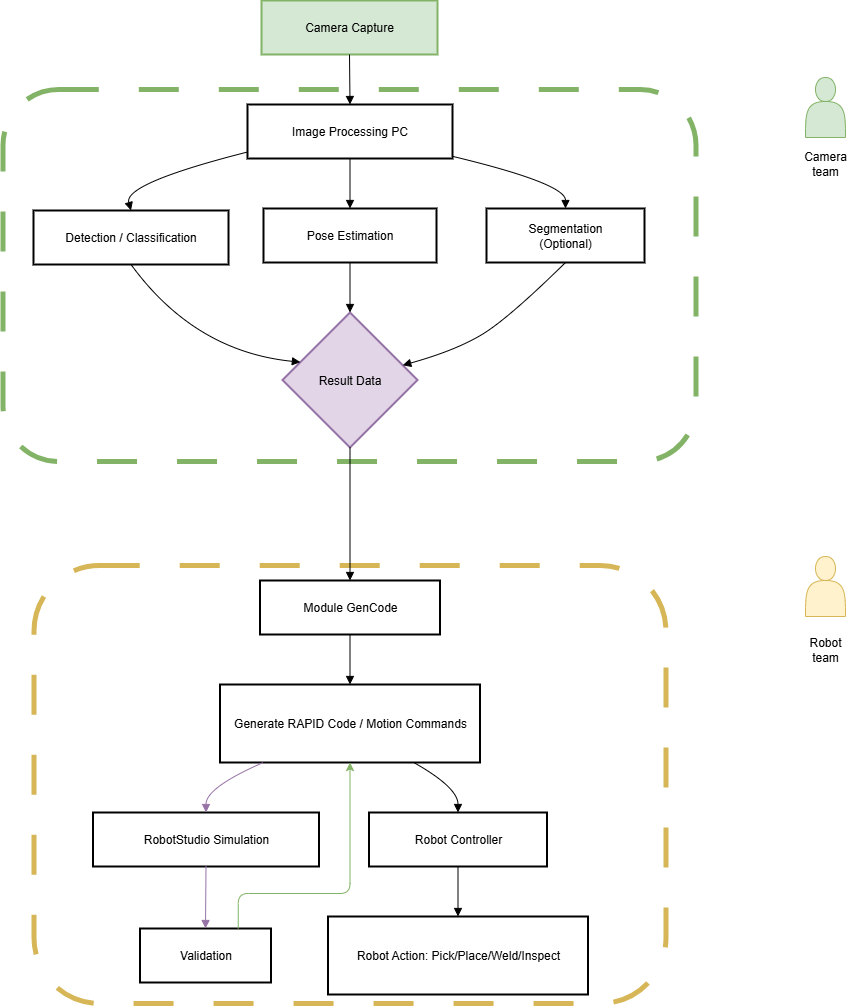
\includegraphics[width= 9cm]{Highflow.png}

\section{Results and Discussion}
\section{Conclusion}

\appendices
\section{Details of the Code Generation Pipeline}
DUMP TEXT

\section{Additional Figures}
DUMP TEXT

\bibliographystyle{IEEEtran}
\bibliography{References}
\vspace{12pt}
\end{document}